\documentclass[english,floatsintext,man]{apa6}

\usepackage{amssymb,amsmath}
\usepackage{ifxetex,ifluatex}
\usepackage{fixltx2e} % provides \textsubscript
\ifnum 0\ifxetex 1\fi\ifluatex 1\fi=0 % if pdftex
  \usepackage[T1]{fontenc}
  \usepackage[utf8]{inputenc}
\else % if luatex or xelatex
  \ifxetex
    \usepackage{mathspec}
    \usepackage{xltxtra,xunicode}
  \else
    \usepackage{fontspec}
  \fi
  \defaultfontfeatures{Mapping=tex-text,Scale=MatchLowercase}
  \newcommand{\euro}{€}
\fi
% use upquote if available, for straight quotes in verbatim environments
\IfFileExists{upquote.sty}{\usepackage{upquote}}{}
% use microtype if available
\IfFileExists{microtype.sty}{\usepackage{microtype}}{}

% Table formatting
\usepackage{longtable, booktabs}
\usepackage{lscape}
% \usepackage[counterclockwise]{rotating}   % Landscape page setup for large tables
\usepackage{multirow}		% Table styling
\usepackage{tabularx}		% Control Column width
\usepackage[flushleft]{threeparttable}	% Allows for three part tables with a specified notes section
\usepackage{threeparttablex}            % Lets threeparttable work with longtable

% Create new environments so endfloat can handle them
% \newenvironment{ltable}
%   {\begin{landscape}\begin{center}\begin{threeparttable}}
%   {\end{threeparttable}\end{center}\end{landscape}}

\newenvironment{lltable}
  {\begin{landscape}\begin{center}\begin{ThreePartTable}}
  {\end{ThreePartTable}\end{center}\end{landscape}}




% The following enables adjusting longtable caption width to table width
% Solution found at http://golatex.de/longtable-mit-caption-so-breit-wie-die-tabelle-t15767.html
\makeatletter
\newcommand\LastLTentrywidth{1em}
\newlength\longtablewidth
\setlength{\longtablewidth}{1in}
\newcommand\getlongtablewidth{%
 \begingroup
  \ifcsname LT@\roman{LT@tables}\endcsname
  \global\longtablewidth=0pt
  \renewcommand\LT@entry[2]{\global\advance\longtablewidth by ##2\relax\gdef\LastLTentrywidth{##2}}%
  \@nameuse{LT@\roman{LT@tables}}%
  \fi
\endgroup}


  \usepackage{graphicx}
  \makeatletter
  \def\maxwidth{\ifdim\Gin@nat@width>\linewidth\linewidth\else\Gin@nat@width\fi}
  \def\maxheight{\ifdim\Gin@nat@height>\textheight\textheight\else\Gin@nat@height\fi}
  \makeatother
  % Scale images if necessary, so that they will not overflow the page
  % margins by default, and it is still possible to overwrite the defaults
  % using explicit options in \includegraphics[width, height, ...]{}
  \setkeys{Gin}{width=\maxwidth,height=\maxheight,keepaspectratio}
\ifxetex
  \usepackage[setpagesize=false, % page size defined by xetex
              unicode=false, % unicode breaks when used with xetex
              xetex]{hyperref}
\else
  \usepackage[unicode=true]{hyperref}
\fi
\hypersetup{breaklinks=true,
            pdfauthor={},
            pdftitle={Untidy Long Paper Example},
            colorlinks=true,
            citecolor=blue,
            urlcolor=blue,
            linkcolor=black,
            pdfborder={0 0 0}}
\urlstyle{same}  % don't use monospace font for urls

\setlength{\parindent}{0pt}
%\setlength{\parskip}{0pt plus 0pt minus 0pt}

\setlength{\emergencystretch}{3em}  % prevent overfull lines

\ifxetex
  \usepackage{polyglossia}
  \setmainlanguage{}
\else
  \usepackage[english]{babel}
\fi

% Manuscript styling
\captionsetup{font=singlespacing,justification=justified}
\usepackage{csquotes}
\usepackage{upgreek}

 % Line numbering
  \usepackage{lineno}
  \linenumbers


\usepackage{tikz} % Variable definition to generate author note

% fix for \tightlist problem in pandoc 1.14
\providecommand{\tightlist}{%
  \setlength{\itemsep}{0pt}\setlength{\parskip}{0pt}}

% Essential manuscript parts
  \title{Untidy Long Paper Example}

  \shorttitle{Untidy}


  \author{Christina Bergmann\textsuperscript{1}~\& The R Unicorn\textsuperscript{2}}

  \def\affdep{{"", ""}}%
  \def\affcity{{"", ""}}%

  \affiliation{
    \vspace{0.5cm}
          \textsuperscript{1} Ecole Normale Superieure\\
          \textsuperscript{2} Institute for Rainbow Studies  }

  \authornote{
    \newcounter{author}
    The authors note that it is quite cold today.

                      Correspondence concerning this article should be addressed to Christina Bergmann, 29, rue d'Ulm. E-mail: \href{mailto:chbergma@gmail.com}{\nolinkurl{chbergma@gmail.com}}
                          }


  \abstract{Enter abstract here (note the indentation, if you start a new
paragraph).}
  \keywords{no keywords \\

    \indent Word count: 666
  }





\begin{document}

\maketitle

\setcounter{secnumdepth}{0}



This sample paper shows how you can combine long texts and code to
generate dynamic journal papers. The following text is taken from
\url{http://barbarplots.github.io} and from
\url{http://cogtales.wordpress.com}. (Note: Adding \url{http://} to URLs
makes them automatically click-able.)

The paper was generated using R (R Core Team, 2016), tidyverse (Wickham,
2016), and papaja (Aust \& Barth, 2016) for formatting the paper in APA
style. You can create citations for R packages using the citation()
command, for example: \texttt{citation("papaja")}.

\subsection{Look, it's a subsection!}\label{look-its-a-subsection}

Data visualization is a complex topic in the experimental sciences.
While there are many ways to display data, many researchers choose to
use bar plots. Generally, these plots only depict a group mean and
standard error (or deviation). Unfortunately, most data are not as clean
as bar plots make them seem, and since bar plots reveal very little
about the distribution of the data, this kind of visualization can be
misleading (Saxon, 2015; Weissgerber, Garovic, Savic, Winham, \& Milic,
2016; Weissgerber, Milic, Winham, \& Garovic, 2015). A further issue is
that of the bar itself, which implies that the base of the y-axis is
meaningful, which is not necessarily the case. The bar can then mislead
readers (Saxon, 2015).

\subsubsection{More on the barbarplots
campaign}\label{more-on-the-barbarplots-campaign}

For the full text with all figures, visit:
\url{https://cogtales.wordpress.com/2016/06/06/congratulations-barbarplots/}

Our kickstarter project \#barbarplots reached its funding goal and will
thus become reality! In the 30-day campaign, 173 backers pledged a total
of 3,479 Euro to send \#barbarplots t-shirts to editors of major
scientific journals. We are very excited and want to thank you for the
tremendous support -- not only by pledging, but also by spreading the
word via email, Facebook, Twitter, and by wearing and carrying tote bags
and t-shirts with the following meme around the world.

We also want to thank everyone that joined the discussion on
\#barbarplots during the 30 days of our campaign. These discussions
happened on people's Facebook pages, in the lab, via email, and on
Twitter. To not lose all these thoughts widespread along the www, I here
try to put together a collection of discussion points -- both critical
thoughts about the campaign itself as well as musings on data
visualization in general. Note that many snippets of answers I borrow
from our British t-shirt doctor Rory, who not only in our video, but
also in real life proved to be the most eloquent \#barbarplots
spokesman.

Before going into it, I want to draw your attention to some of the the
shoulders this campaign is standing on, for instance Weissgerber et al.
(2015), who started the plotting revolution much earlier.

So off we go -- I'll start with the maybe most obvious critical remark
about our campaign.

\paragraph{But barplots can be a good way to
plot!}\label{but-barplots-can-be-a-good-way-to-plot}

Sure. That's why we used the following barplot for the cost breakdown of
our kickstarter project to demonstrate that count data with a meaningful
zero and no distributional properties can be wonderfully represented by
a barplot.

This explanation, however, quite readily leads to critique number 2:

\paragraph{But why do you say \#barbarplots if you do not actually mean
it??}\label{but-why-do-you-say-barbarplots-if-you-do-not-actually-mean-it}

Some people pointed out that our hashtag \#barbarplots, our slogan
\enquote{Friends don't let friends make barplots} and our campaign video
with the cats-and-dogs example were catchy but partially misleading.

That's true. But we made a conscious decision in favor of catchiness and
simplicity in order to increase the likelihood people would raise their
head and smile and share. Researchers take their work seriously and
details are important, but they're also humans with an often already
overstrained attention span. And they're also smart enough to look
beyond the (attention-catching) headline to ponder the more nuanced
argument.

We are aware that some people might still be misled by the simplified
version of our message, and could even religiously stop using barplots
no matter what. But this is, for sure, not a problem that our slogan is
causing.

\paragraph{What are cases in which barplots are not good and
why?}\label{what-are-cases-in-which-barplots-are-not-good-and-why}

In general, we consider barplots not to be the most informative way to
represent distributional data. For example, perhaps an effect is driven
entirely by a subset of participants in the experiment? Perhaps a null
effect arises because some participants have a negative effect and
others have a positive effect? Perhaps some items are extremely
variable? Perhaps the data are very non-normal and using inferential
statistics is inappropriate? And even if your data are perfectly
normally distributed, wouldn't it make your paper even more convincing
if your visualization method reflected that?

\paragraph{Ok, so what you want to say is that we should not be
comparing
means?}\label{ok-so-what-you-want-to-say-is-that-we-should-not-be-comparing-means}

It is true that the issue of barplots as a data visualisation technique
often goes together with the issue of doing statistics by comparing
means. However, they are nevertheless separate issues. The focus of the
campaign is really about barplots as a visualization technique. We just
want to make sure that we think about the choice rather than
formulaically applying one way of analysis or visualization.

\paragraph{So\ldots{}what IS a better plot to represent
distributions?}\label{sowhat-is-a-better-plot-to-represent-distributions}

In our campaign, we promote box plots and histograms. Both tell us way
more about the distribution of data than barplots, notably about the
spread and skewness of the underlying data. And there's more: Scatter
plots, violin plots, swarm plots, pirate plots. Below is an example of
how the same data would look with different types of plots.

Though this is not the case in the above graphs, the way we plotted in
our original meme lead some people to say:

\paragraph{Your histogram has two x axes!! That is very
misleading!}\label{your-histogram-has-two-x-axes-that-is-very-misleading}

It is true that the histogram differs from the other plots in this
aspect. Sure, we could have superimposed the distributions so that there
was only one x axis (but then the plot would differ from the others in
the sense that it would not be a side-by-side but an overlaid
representation). We could have also rotated the histogram 90 degrees to
make the y axes match (but then it would differ from the others by being
vertically as opposed to horizontally aligned). In short: Yes, there
would have been other ways to do it, but it is not clear that there was
a clearly better way to do it. Also, we do not want to promote boxplots
or histograms as a single alternative to barplots (see above) -- all we
want is for us to think about our choices.

Still, we want to emphasize that a barplot is often not the most
informative alternative for distributional data. That leads me to the
last frequent point of criticism:

\paragraph{Isn't a plot supposed to be an abstraction of the data and a
means to present them in the simplest and most understandable way
possible?}\label{isnt-a-plot-supposed-to-be-an-abstraction-of-the-data-and-a-means-to-present-them-in-the-simplest-and-most-understandable-way-possible}

To that, I would first want to state the obvious that simple isn't
always good. Like interpreting everything below p = .05 as a victory and
above as an epic failure. It's not good, it's not right, and part of its
being simple is certainly convention and habitude.

But still, a summary/abstraction/simplification of the raw data cannot
be a bad idea to bring your point across? This question gets at the
heart of what visualization is for and what scientific publishing is
supposed to do. If the visualization is to be as simple as possible to
get the most basic point across, maybe just showing means is fine. (To
be honest, though, if you're just reporting two means, don't waste space
with a graph, just put that in the text.) However, it's conventional for
us to go into a lot of obsessive detail in our reporting of methods and
statistical analyses -- so why not with our graphs too? Showing or
summarizing the distribution can be a useful way to put your cards on
the table for readers to see that you are not trying to hide or
obfuscate any unusual outliers or strange trends.

But of course, if we're giving a 10-min-talk in front of an audience
that is used to barplots, walking the audience through the graph would
require more time than you have.

Luckily, there are many compromises that can be made -- for example,
plot a grand mean, along with (less visually prominent) subject means,
so that the variability in the data is more apparent. Or a boxplot,
which is visually less dense than other alternatives to barplots.

In summary\ldots{}

Thank you again to all of our backers, tweeters, and reposters. We've
really enjoyed working on this campaign, from filming the video to group
discussions on and off social media. The campaign is by no means over
though, so look for updates as we complete our aim to send out t-shirts
to journal editors and continue the discussion. Happy plotting!

Your \#barbarplots team,

Page Piccinini,\\
Christina Bergmann,\\
Sho Tsuji,\\
Alexander Martin,\\
Rory Turnbull,\\
Adriana Guevara Rukoz,\\
M. Julia Carbajal

\section{Methods}\label{methods}

The data I am using here comes with R and is called Anscombe's Quartet.

\subsection{Wikipedia description of Anscombe's
Quartet}\label{wikipedia-description-of-anscombes-quartet}

source: \url{https://en.wikipedia.org/wiki/Anscombe's_quartet}

Anscombe's quartet comprises four datasets that have nearly identical
simple descriptive statistics, yet appear very different when graphed.
Each dataset consists of eleven (x,y) points. They were constructed in
1973 by the statistician Francis Anscombe to demonstrate both the
importance of graphing data before analyzing it and the effect of
outliers on statistical properties. He described the article as being
intended to attack the impression among statisticians that
\enquote{numerical calculations are exact, but graphs are rough.}
(Anscombe, 1973)

The quartet is still often used to illustrate the importance of looking
at a set of data graphically before starting to analyze according to a
particular type of relationship, and the inadequacy of basic statistic
properties for describing realistic datasets

\section{Results}\label{results}

\subsection{Descriptive Statistics}\label{descriptive-statistics}

We're now preparing a table by creating a data structure that has
exactly the fields we want to display, plus column headers. For advanced
users, you can also modify the column headers and other parts of how
this table turns out. The second table is showing the same data, but
instead of using the APA format, it is generated using kable.

\begin{table}[tbp]
\begin{center}
\begin{threeparttable}
\caption{Descriptive statistics of Anscombe's quartet.}
\begin{tabular}{lll}
\toprule
key & \multicolumn{1}{c}{mean} & \multicolumn{1}{c}{sd}\\
\midrule
y1 & 7.500909 & 2.031568\\
y2 & 7.500909 & 2.031657\\
y3 & 7.500000 & 2.030424\\
y4 & 7.500909 & 2.030579\\
\bottomrule
\end{tabular}
\begin{tablenotes}[para]
\textit{Note.} This table was created with apa\_table()
\end{tablenotes}
\end{threeparttable}
\end{center}
\end{table}

Let's talk a bit about the statistics. So it looks like all means and
sds are quite similar. That's part of the point Anscombe (1973) was
making.

\begin{tabular}{l|r|r}
\hline
key & mean & sd\\
\hline
y1 & 7.500909 & 2.031568\\
\hline
y2 & 7.500909 & 2.031657\\
\hline
y3 & 7.500000 & 2.030424\\
\hline
y4 & 7.500909 & 2.030578\\
\hline
\end{tabular}

\subsection{Data Visualization}\label{data-visualization}

First, because this paper is based on a \#barbarplots talk I gave last
summer, here is of course one of those odious barplots! Look, all
datasets look the same! Quelle horreur!

\begin{figure}[htbp]
\centering
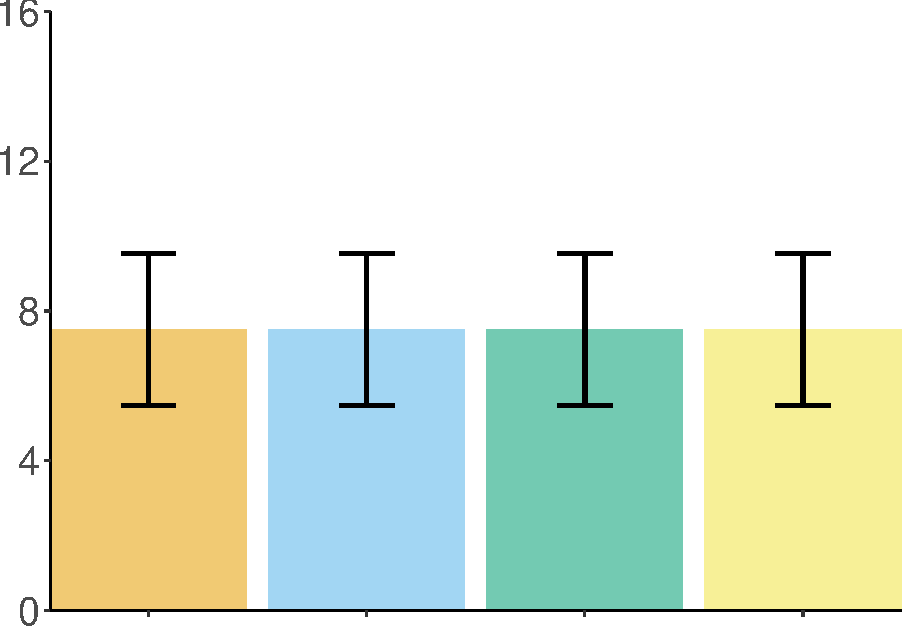
\includegraphics{APA_Untidy_Paper_files/figure-latex/unnamed-chunk-1-1.pdf}
\caption{\label{fig:unnamed-chunk-1}Barplots of one dimension of Anscombe's
Quartet}
\end{figure}

Next, we want to look at some boxplots. Look, some differences between
the datasets become visible.

\begin{figure}[htbp]
\centering
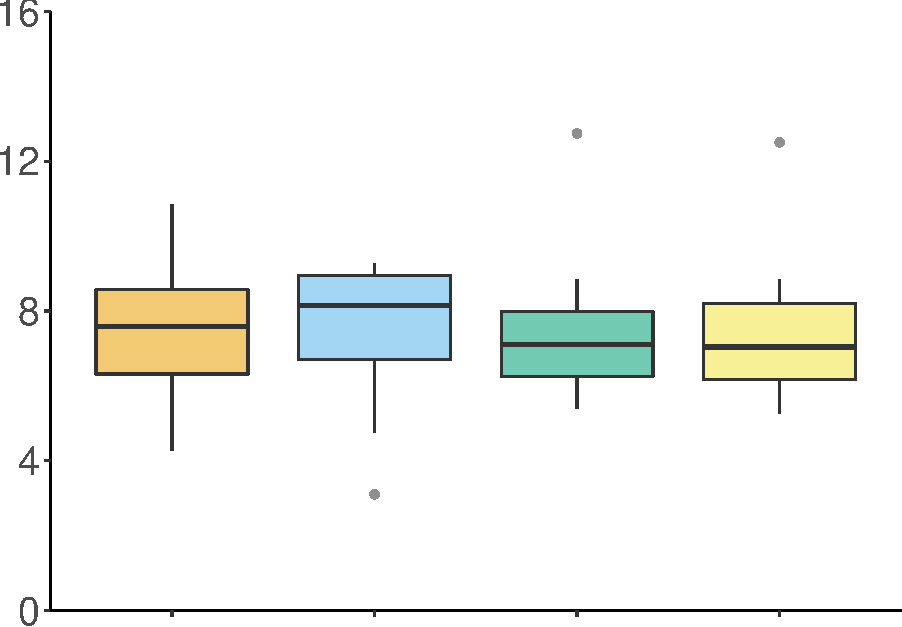
\includegraphics{APA_Untidy_Paper_files/figure-latex/unnamed-chunk-2-1.pdf}
\caption{\label{fig:unnamed-chunk-2}The same data as before in a boxplot.}
\end{figure}

\subsection{Plotting both dimensions of the famous
Quartet}\label{plotting-both-dimensions-of-the-famous-quartet}

\begin{figure}[htbp]
\centering
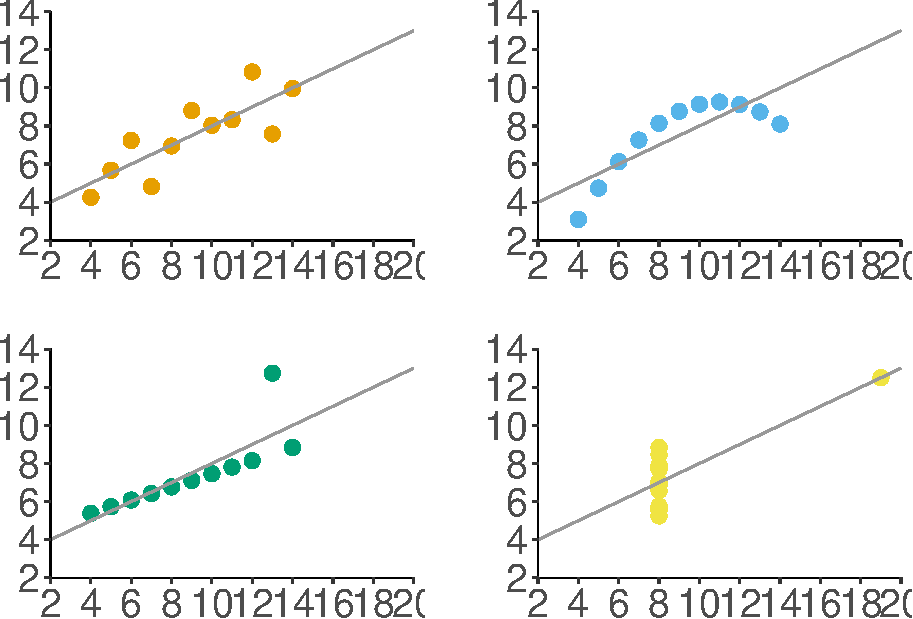
\includegraphics{APA_Untidy_Paper_files/figure-latex/unnamed-chunk-3-1.pdf}
\caption{\label{fig:unnamed-chunk-3}The classical Anscombe Quartet plot. All
means and correlations are the same, but the raw data differ quite a
bit.}
\end{figure}

The first scatter plot (top left) appears to be a simple linear
relationship, corresponding to two variables correlated and following
the assumption of normality. The second graph (top right) is not
distributed normally; while an obvious relationship between the two
variables can be observed, it is not linear, and the Pearson correlation
coefficient is not relevant (a more general regression and the
corresponding coefficient of determination would be more appropriate).
In the third graph (bottom left), the distribution is linear, but with a
different regression line, which is offset by the one outlier which
exerts enough influence to alter the regression line and lower the
correlation coefficient from 1 to 0.816 (a robust regression would have
been called for). Finally, the fourth graph (bottom right) shows an
example when one outlier is enough to produce a high correlation
coefficient, even though the relationship between the two variables is
not linear.

\newpage 

\subsection{Let's do some stats}\label{lets-do-some-stats}

\begin{verbatim}
## 
## Call:
## lm(formula = anscombe$x3 ~ anscombe$y3)
## 
## Residuals:
##     Min      1Q  Median      3Q     Max 
## -2.9869 -1.3733 -0.0266  1.3200  3.2133 
## 
## Coefficients:
##             Estimate Std. Error t value Pr(>|t|)   
## (Intercept)  -1.0003     2.4362  -0.411  0.69097   
## anscombe$y3   1.3334     0.3145   4.239  0.00218 **
## ---
## Signif. codes:  0 '***' 0.001 '**' 0.01 '*' 0.05 '.' 0.1 ' ' 1
## 
## Residual standard error: 2.019 on 9 degrees of freedom
## Multiple R-squared:  0.6663, Adjusted R-squared:  0.6292 
## F-statistic: 17.97 on 1 and 9 DF,  p-value: 0.002176
\end{verbatim}

\begin{verbatim}
## 
## Call:
## lm(formula = anscombe$x4 ~ anscombe$y4)
## 
## Residuals:
##     Min      1Q  Median      3Q     Max 
## -2.7859 -1.4122 -0.1853  1.4551  3.3329 
## 
## Coefficients:
##             Estimate Std. Error t value Pr(>|t|)   
## (Intercept)  -1.0036     2.4349  -0.412  0.68985   
## anscombe$y4   1.3337     0.3143   4.243  0.00216 **
## ---
## Signif. codes:  0 '***' 0.001 '**' 0.01 '*' 0.05 '.' 0.1 ' ' 1
## 
## Residual standard error: 2.018 on 9 degrees of freedom
## Multiple R-squared:  0.6667, Adjusted R-squared:  0.6297 
## F-statistic:    18 on 1 and 9 DF,  p-value: 0.002165
\end{verbatim}

As suggested by the plots, the linear models are very similar (the
correlations even more so). We can also report results in line, for
example the \emph{p}-value = 0.00. Note that this number is really not
correct, because it is rounded to two digits!

\newpage

\section{References}\label{references}

\setlength{\parindent}{-0.5in} \setlength{\leftskip}{0.5in}

\hypertarget{refs}{}
\hypertarget{ref-Anscombe}{}
Anscombe, F. J. (1973). Graphs in statistical analysis. \emph{The
American Statistician}, \emph{27}(1), 17--21.

\hypertarget{ref-R-papaja}{}
Aust, F., \& Barth, M. (2016). \emph{Papaja: Create apa manuscripts with
rmarkdown}. Retrieved from \url{https://github.com/crsh/papaja}

\hypertarget{ref-R-base}{}
R Core Team. (2016). \emph{R: A language and environment for statistical
computing}. Vienna, Austria: R Foundation for Statistical Computing.
Retrieved from \url{https://www.R-project.org/}

\hypertarget{ref-Saxon}{}
Saxon, E. (2015). Beyond bar charts. \emph{BMC Biology}, \emph{13}(1),
60.

\hypertarget{ref-Weissgerber2016}{}
Weissgerber, T. L., Garovic, V. D., Savic, M., Winham, S. J., \& Milic,
N. M. (2016). From static to interactive: Transforming data
visualization to improve transparency. \emph{PLoS Biology},
\emph{14}(6), e1002484.

\hypertarget{ref-Weissgerber2015}{}
Weissgerber, T. L., Milic, N. M., Winham, S. J., \& Garovic, V. D.
(2015). Beyond bar and line graphs: Time for a new data presentation
paradigm. \emph{PLoS Biology}, \emph{13}(4), e1002128.

\hypertarget{ref-R-tidyverse}{}
Wickham, H. (2016). \emph{Tidyverse: Easily install and load 'tidyverse'
packages}. Retrieved from
\url{https://CRAN.R-project.org/package=tidyverse}






\end{document}
